%%%%%%%%%%%%%%%%%%%%%%%%%%%%%%%%%%%%%%%% DECLARATION %%%%%%%%%%%%%%%%%%%%%%%%%%%%%%%%%%%%%%%%
\documentclass[12pt,czech]{article}
\usepackage{graphicx}
\usepackage[T1]{fontenc}
%\usepackage{babel}
\usepackage[utf8]{inputenc} % set coding
\usepackage{czech}
\usepackage[legalpaper, portrait, margin=0.6in]{geometry}
\usepackage{fixltx2e}
\usepackage{hyperref}
\usepackage{textgreek}
\usepackage{textcomp}
\usepackage{adjustbox}
\usepackage{float}

\usepackage{listings}
\usepackage{color}

\definecolor{dkgreen}{rgb}{0,0.6,0}
\definecolor{gray}{rgb}{0.5,0.5,0.5}
\definecolor{mauve}{rgb}{0.58,0,0.82}

\lstset{frame=tb,
  language=Python,
  aboveskip=3mm,
  belowskip=3mm,
  showstringspaces=false,
  columns=flexible,
  basicstyle={\small\ttfamily},
  numbers=none,
  numberstyle=\tiny\color{gray},
  keywordstyle=\color{blue},
  commentstyle=\color{dkgreen},
  stringstyle=\color{mauve},
  breaklines=true,
  breakatwhitespace=true,
  tabsize=3
}

\author{
  Šesták, Pavel\\
  \texttt{xsesta07@stud.fit.vutbr.cz}
}

\title{ISS Projekt}
\date{13.12.2020}  


%%%%%%%%%%%%%%%%%%%%%%%%%%%%%%%%%%%%%%%% TITLE PAGE %%%%%%%%%%%%%%%%%%%%%%%%%%%%%%%%%%%%%%%%
\begin{document}
  \begin{titlepage}
		\begin{center}
			%\textsc{\LARGE Vysoké Učení Technické v Brně} \\[0.5cm]
			%{\LARGE Fakulta informačních technologií}

			\begin{figure}
				\center
\includegraphics[scale=0.3]{images/logo.png}
			\end{figure}

			\vspace{3cm}

			\textsc{\LARGE Signály a systémy } \\[0.5cm]
			\textsc{\LARGE 2020/2021} \\[3.5cm]

			\textbf{\LARGE ISS Projekt - Protokol} \\
		    \vspace{3cm}
		    
		    {\Large Šesták Pavel(xsesta07)} \\[0.5cm]
			
			\vspace{3cm}
                
		    \textsc{}{\LARGE Brno, \today}

		\end{center}
	\end{titlepage}

%%%%%%%%%%%%%%%%%%%%%%%%%%%%%%%%%%%%%%%% CONTENT TABLE %%%%%%%%%%%%%%%%%%%%%%%%%%%%%%%%%%%%%%%%
\begin{center}
	\tableofcontents %content generate
	\clearpage %end of page
\end{center}

%%%%%%%%%%%%%%%%%%%%%%%%%%%%%%%%%%%%%%%% SECTION INPUT SIGNALS %%%%%%%%%%%%%%%%%%%%%%%%%%%%%%%%%%%%%%%%
\section{Tabulka vstupních signálů}¨

\begin{table}[H]
\begin{tabular}{|l|l|l|}
\hline
Název nahrávky                          & Délka nahrávky{[}s{]}      & Počet vzorků                \\ \hline
\multicolumn{1}{|l|}{maskoff\_tone}     & \multicolumn{1}{l|}{01.00} & \multicolumn{1}{l|}{16000} \\ \hline
\multicolumn{1}{|l|}{maskon\_tone}      & \multicolumn{1}{l|}{01.00} & \multicolumn{1}{l|}{16000} \\ \hline
\multicolumn{1}{|l|}{maskoff\_sentence} & \multicolumn{1}{l|}{05.56} & \multicolumn{1}{l|}{89036} \\ \hline
maskon\_sentence                        & 05.84                      & 93413                      \\ \hline
\end{tabular}
\end{table}

%%%%%%%%%%%%%%%%%%%%%%%%%%%%%%%%%%%%%%%% SECTION FRAMES %%%%%%%%%%%%%%%%%%%%%%%%%%%%%%%%%%%%%%%%
\section{Úloha 3 - Rámce}
    Vstupní signály byly ustředněny a normaliyzovány do dynamického rozsahu [-1;1]\newline
    Frekvence vstupního signálu je 16Khz, podělením dostaneme počet vzorků (samples) na 1ms\newline
    \[f = 16KHz => 1ms = 16\]\newline
    1 milisekunda odpovídá 16 vzorkům vstupního signálu\newline \newline
    1 rámec (frame) je dlouhý 20ms, vynásobením předchozí hodnoty získáme počet vzorků v rámci\\
    \[ 20ms = 20*16 = 320 \]\\
    Výsledná délka rámce je tedy 320 vzorků \newline \newline
    Rámce se vždy polovinou své délky překrývají, nyní vypočítáme počet rámců na 16 000 vzorků \newline
    \[samples/(frame/2) = 16000/160 = 100 \] \\
    Poslední rámec se již nevleze do 1s celý, pouze jeho polovina, z tohoto důvodu dále uvažujeme pouze 99 rámců
    
    \begin{center}
        18. rámec signálu bez roušky a s rouškou
        \hfill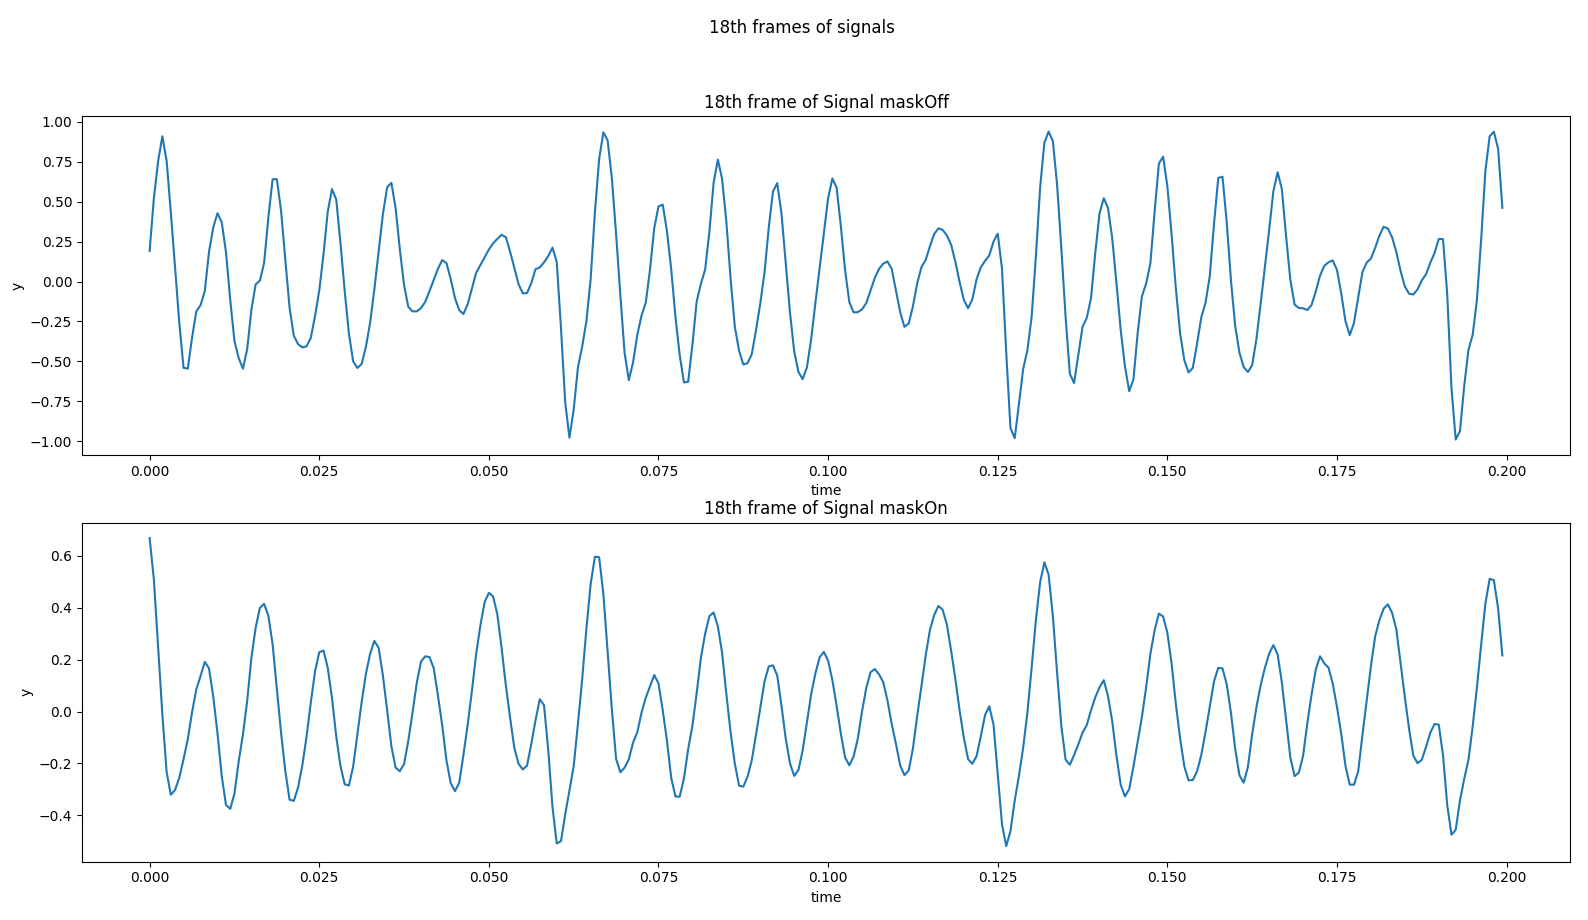
\includegraphics[scale=0.48]{images/18thframe.png}\hspace*{\fill}
    \end{center}
\clearpage

\section{Úloha 4 - základní frekvence rámců }
    Z předchozí úlohy jsme zjistili že máme 99 rámců a každý rámec obsahuje 320 hodnot. Nyní bude demonstrován výpočet základní frekvence 18 tého rámce. Pro získání grafu základních frekvencí je nutné výpočet provést pro každý rámec.
    
    \subsection{Centrální klipování s 70\% práhem}
        Pro výpočet centrálního klipování musíme najít hodnotu práhu P s kterou budeme následně vzorky porovnávat
        \[ P = max(abs(frame))*0.7\]
        Následně provedeme porovnání pro každý vzorek v rámci a v případě že hodnota je větší než P pak hodnotu nastavíme na 1, v případě že hodnota je menší než -1*P pak nastavíme na -1 v ostatních případech bude hodnota rovna 0.
        \begin{center}
            18. rámec po centrálním klipování
            \hfill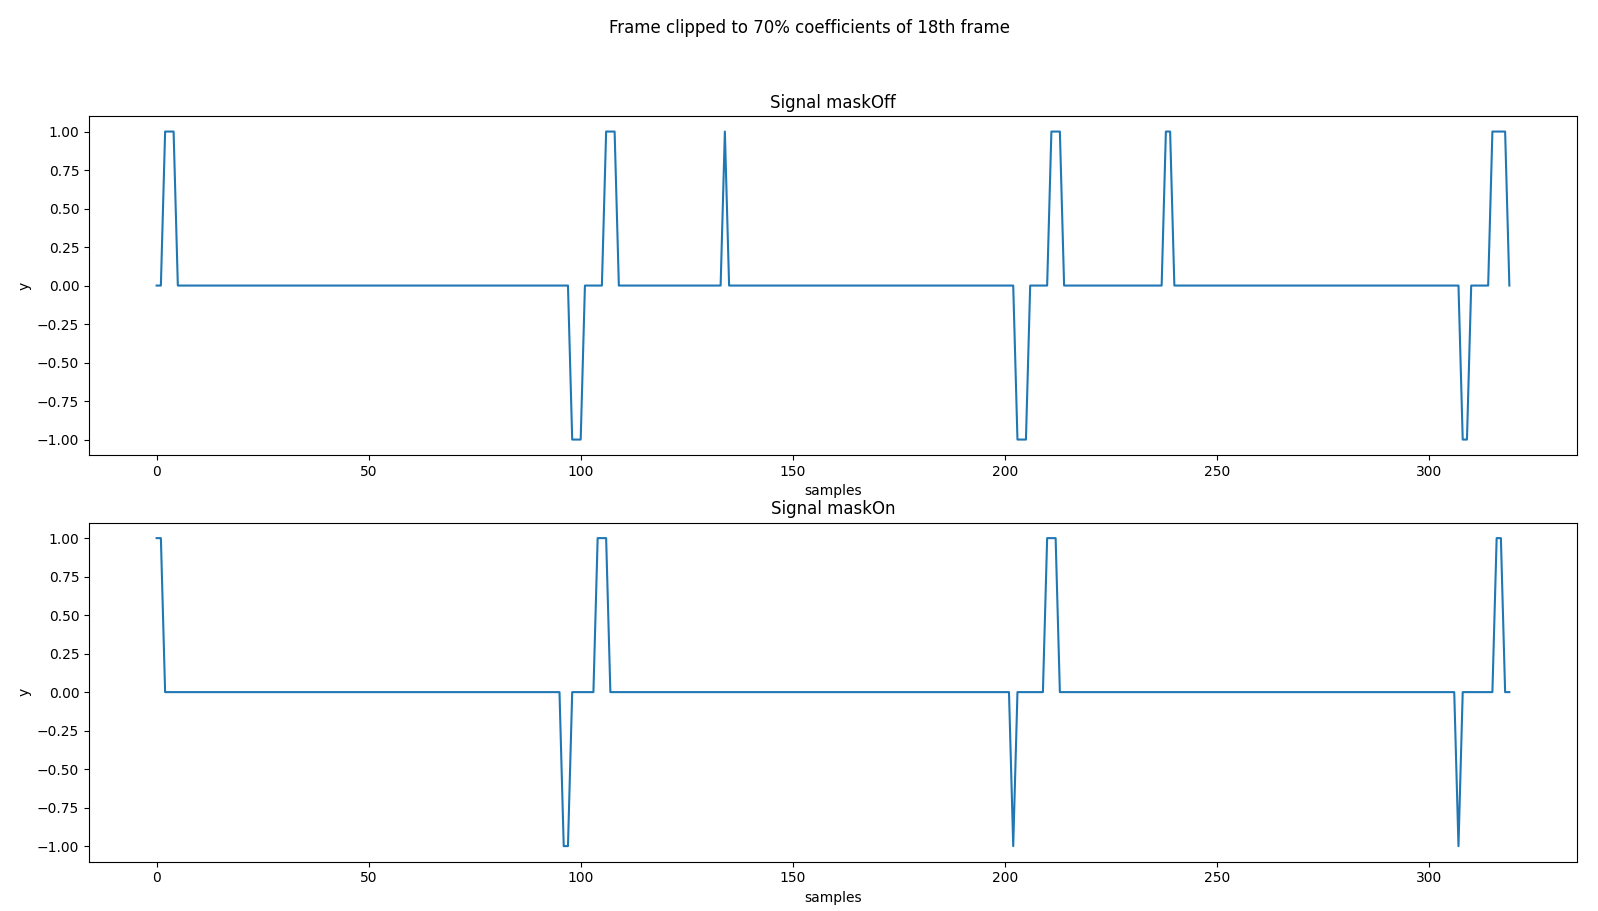
\includegraphics[scale=0.48]{images/18thframe_clipping.png}\hspace*{\fill}
        \end{center}
    \clearpage
    \subsection{Autokorelace rámců}
        Nyní provedeme autokorelaci na signál, který jsme získali centrálním klipováním
        \[ R(k) = \sum_{0}^{N-k} s[k]s[k+n] \]
        Autokorelace nám vyjde vysoká u nuly, protože každý signál je podobný sám na sebe. Proto si určíme práh (trashold), od kterého budeme hledat maximální hodnotu neboli lag. Index práhu v projektu je určován prvním výskytem hodnoty 0 v signálu a následně inkrementován o 1.
        \begin{center}
            18. rámec po autokorelaci
            \hfill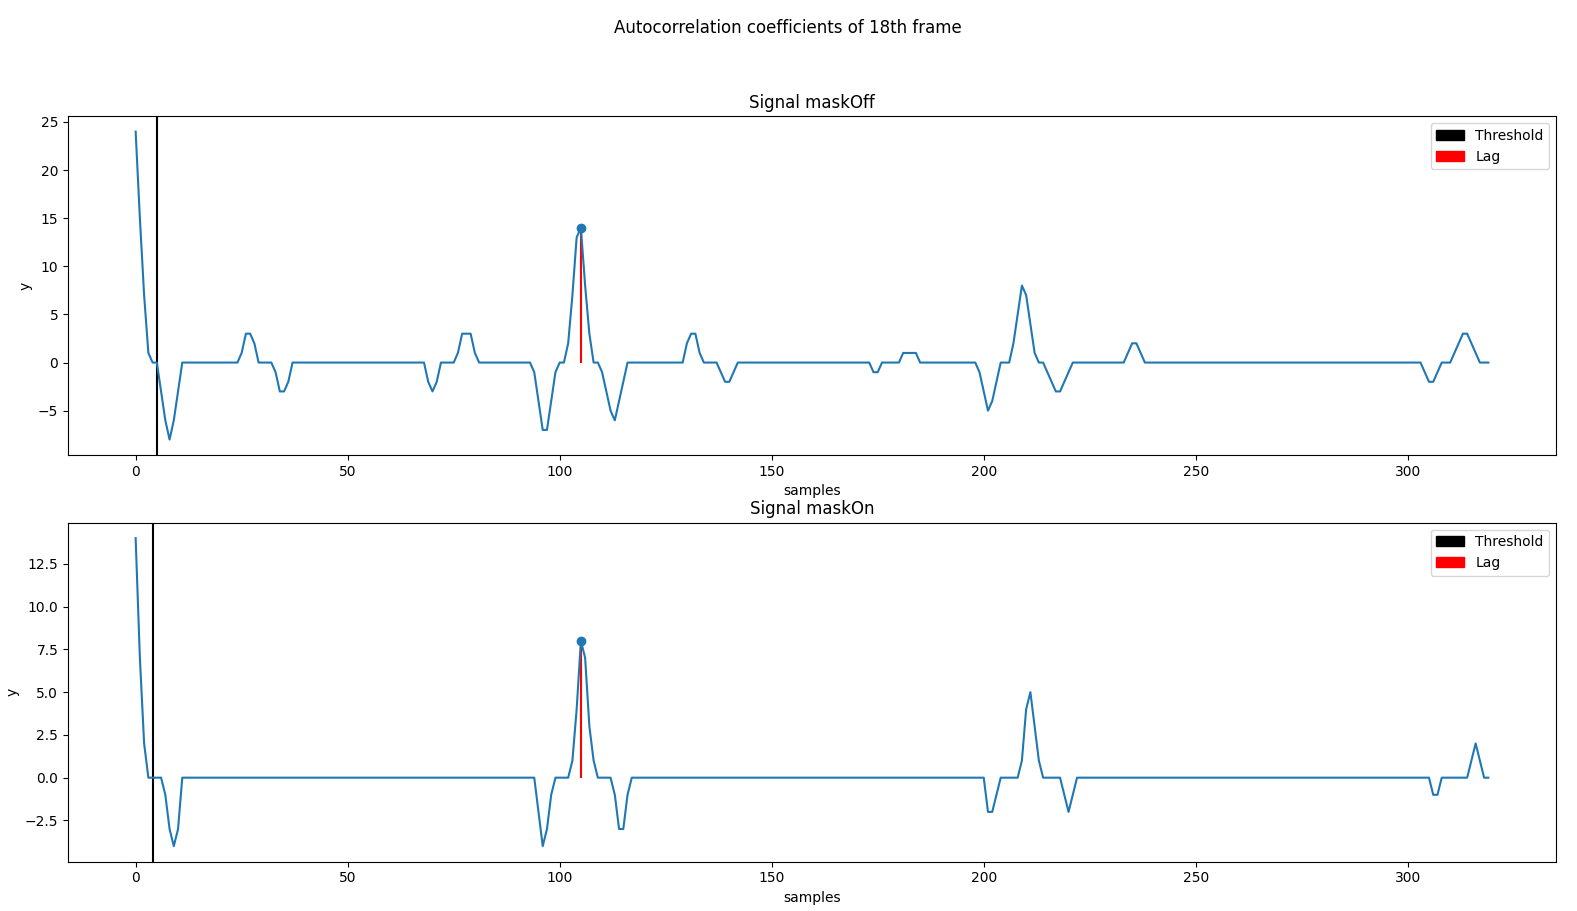
\includegraphics[scale=0.48]{images/18thframe_autocorrelation.png}\hspace*{\fill}
        \end{center}
    \clearpage
    \subsection{Základní frekvence rámců}
        Z předchozího výpočtu jsme získali koeficient lagu. Nyní vyjdeme z těchto vztahů\\
        \\Perioda základního tónu je dána vztahem:\\
        \[T_0 = \frac{1}{F_0} \]
        \\Lag je dán vztahem: \\
        \[L = T_0 F_S \]
        \\Po výpočtu autokorelace jsme získali hodnotu L, hodnota F\textsubscript{S} je vzorkovací frekvence dána signálem
        Nyní vyjádříme F\textsubscript{0}
        \[F_0 = \frac{F_S}{L}\]
        Z důvodu že F\textsubscript{S} je dost vysoké číslo (řádově nižší desítky tisíc) a L je hodnota okolo 100 tak velký rozdíl mezi těmito hodnotami při změně L o +- 1 způsobí velký rozdíl ve změně frekvence. Snížení změn by se docílilo snížením vzorkovací frekvence.\newline\newline
        Střední hodnota pro signál bez roušky: 149.0136\\
        Střední hodnota pro signál s rouškou: 149.5713\\
        Rozptyl pro signál bez roušky:  1.5196\\
        Rozptyl pro signál s rouškou: 1.5196\\
        
        \begin{center}
            Frekvence rámců
            \hfill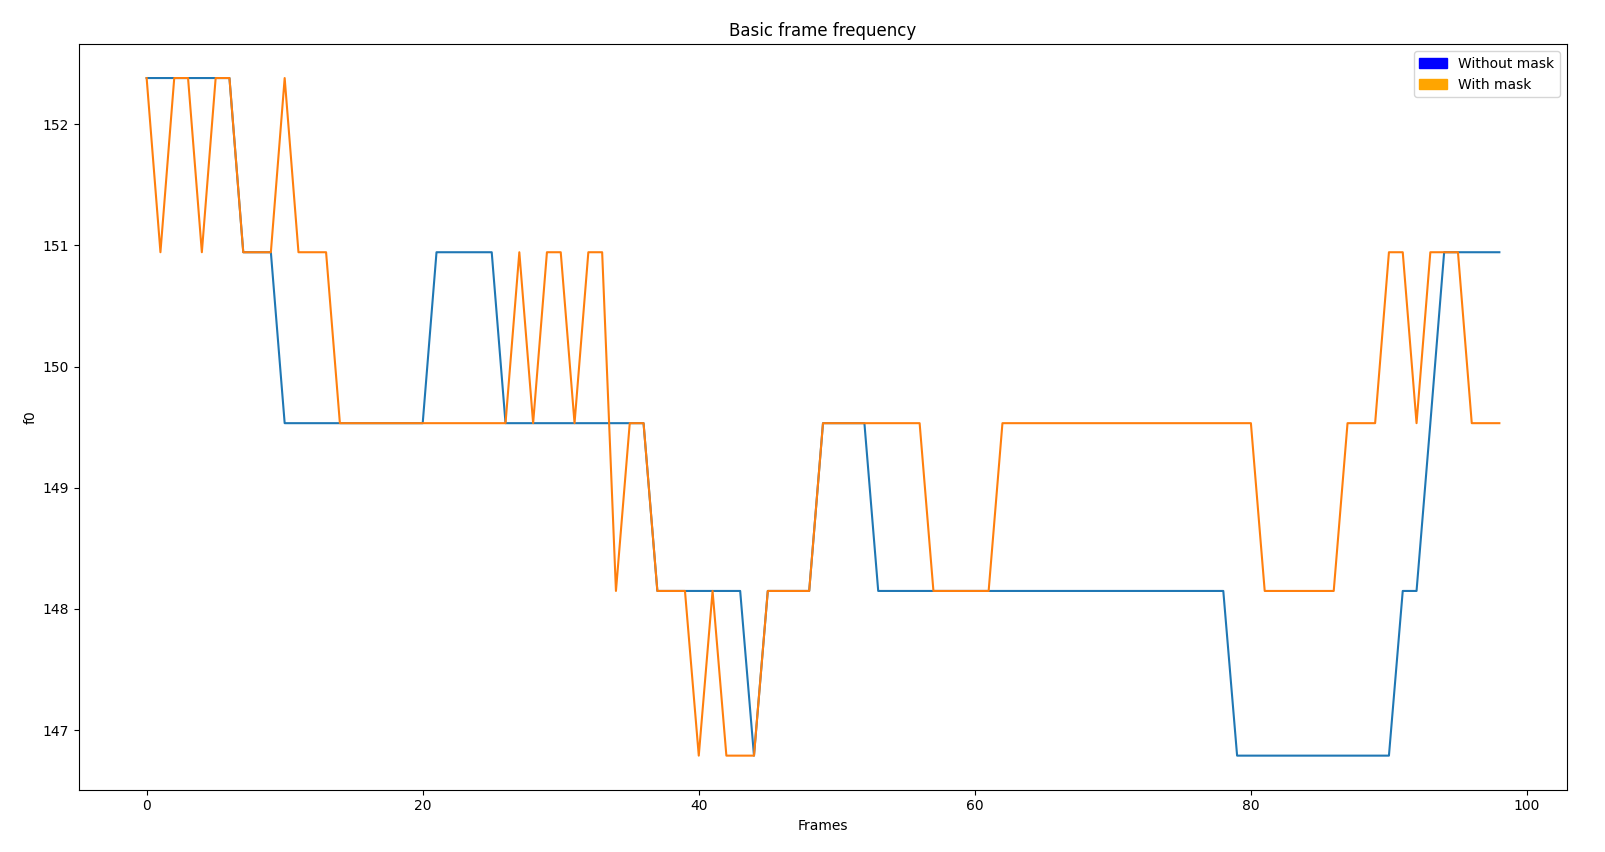
\includegraphics[scale=0.45]{images/freq0.png}\hspace*{\fill}
        \end{center}
\clearpage
\section{Úloha 5 - Spektrogramy}
\subsection{Diskrétní Fourierova transformace}
Pro výpočet spektrogramu budeme potřebovat vypočítat DFT.\newline 
Vzorec pro výpočet DFT:
\[X[k] = \sum_{n = 0}^{N - 1} x[n] e^{-j2\pi\frac{k}{N}n}\]
Implementace DFT:
\begin{lstlisting}
 for i in range(SIGNAL_COUNT):
        for frame_id in range(FRAMES_COUNT):
            print("Frame ",frame_id)#checking status (very long operation)
            for k in range(N):
                for n in range(SAMPLES_IN_FRAME):
                    X[i][frame_id][k] += frames[i][frame_id][n]*(np.exp(-1j*2*np.pi*(k/N)*n))
\end{lstlisting}

V rámci matematických knihoven, v našem případě numpy, je možno volat numpy.fft.fft(signal). FFT neboli rychlá Fourierova transformace patří k nejvýznamnějším algoritmům na světě a významně urychluje výpočet DFT. Implementace základní DFT je velmi časově náročná a výpočet trvá v řádu minut.

\subsection{Logaritmický výkonový spektrogram}
    Koeficienty získané pomocí DFT je nyní nutné upravit na výkon.
    \[P[k] = 20log_{10}|X[k]|\]
    Následně necháme vykreslit spektrogram
    \begin{center}
        \hfill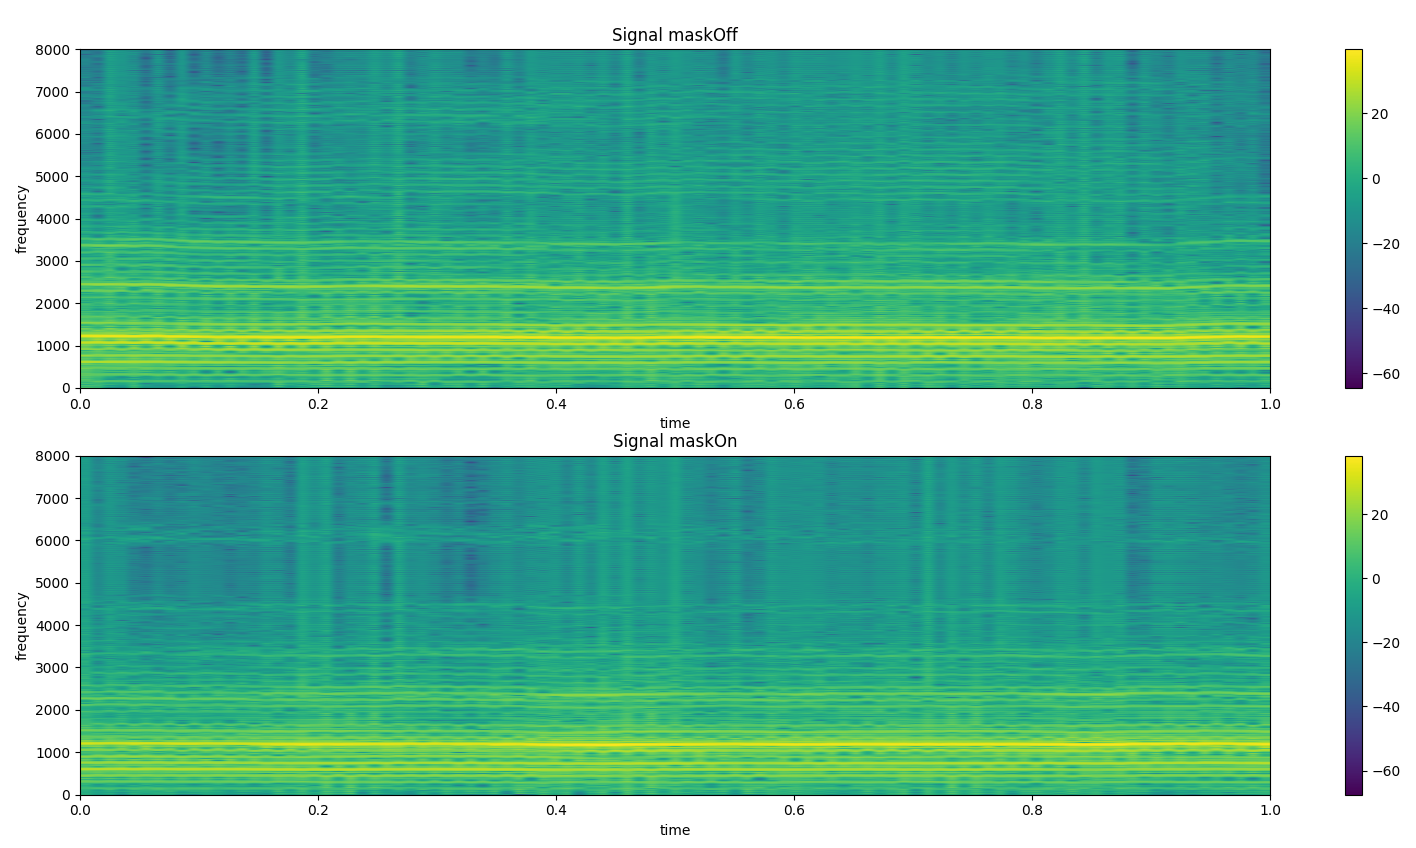
\includegraphics[scale=0.48]{images/spectrums.png}\hspace*{\fill}
    \end{center}
\clearpage
\section{Úloha 6 - Frekvenční charakteristika roušky}
    Frekvenční charakteristika je dána následujícím vztahem:
    
        \[H(e^{j\omega}) = \frac{\sum_{k = 0}^{M} Y[k]e^{-j\omega k}}
                                {\sum_{l = 0}^{N} X[k]e^{-j\omega k}} \]
    
    Výsledná frekvenční charakteristika:
    \begin{center}
        \hfill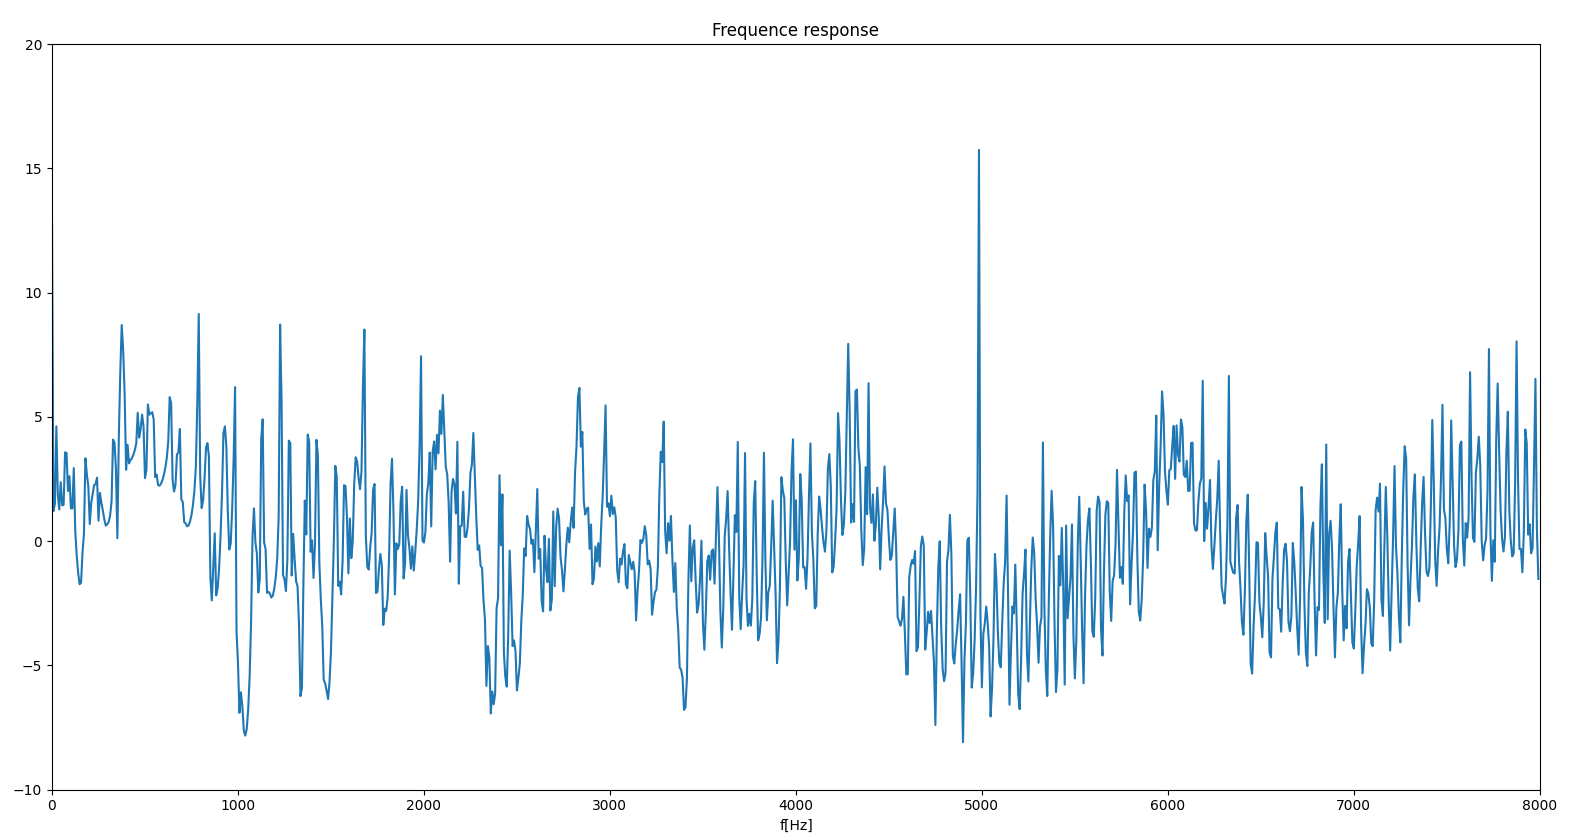
\includegraphics[scale=0.45]{images/frequence_response.png}\hspace*{\fill}
    \end{center}
    Z frekvenční charakteristiky filtru nelze jednoznačně popsat o jaký typ filtru se jedná. Vidíme například potlačení frekvence okolo 1KHz.
\clearpage
\section{Úloha 7 - Impulzní odezva}
Aplikací inverzní diskrétní Fourierovy transformace(IDFT) na frekvenční charakteristiku dostaneme impulzní odezvu.\newline
Vzorec pro výpočet IDFT:
    \[x[n] = \frac{1}{N} \sum_{k = 0}^{N - 1}X[k] e^{j2\pi\frac{k}{N}n}\]
Implementace IDFT:
\begin{lstlisting}
 for n in range(N): 
        for k in range(N):
            h[n] += HjwAvg[k]*(np.exp(1j*2*np.pi*(k/N)*n))
        h[n] /= N
\end{lstlisting}
Graf impulzní odezvy:
\begin{center}
\hfill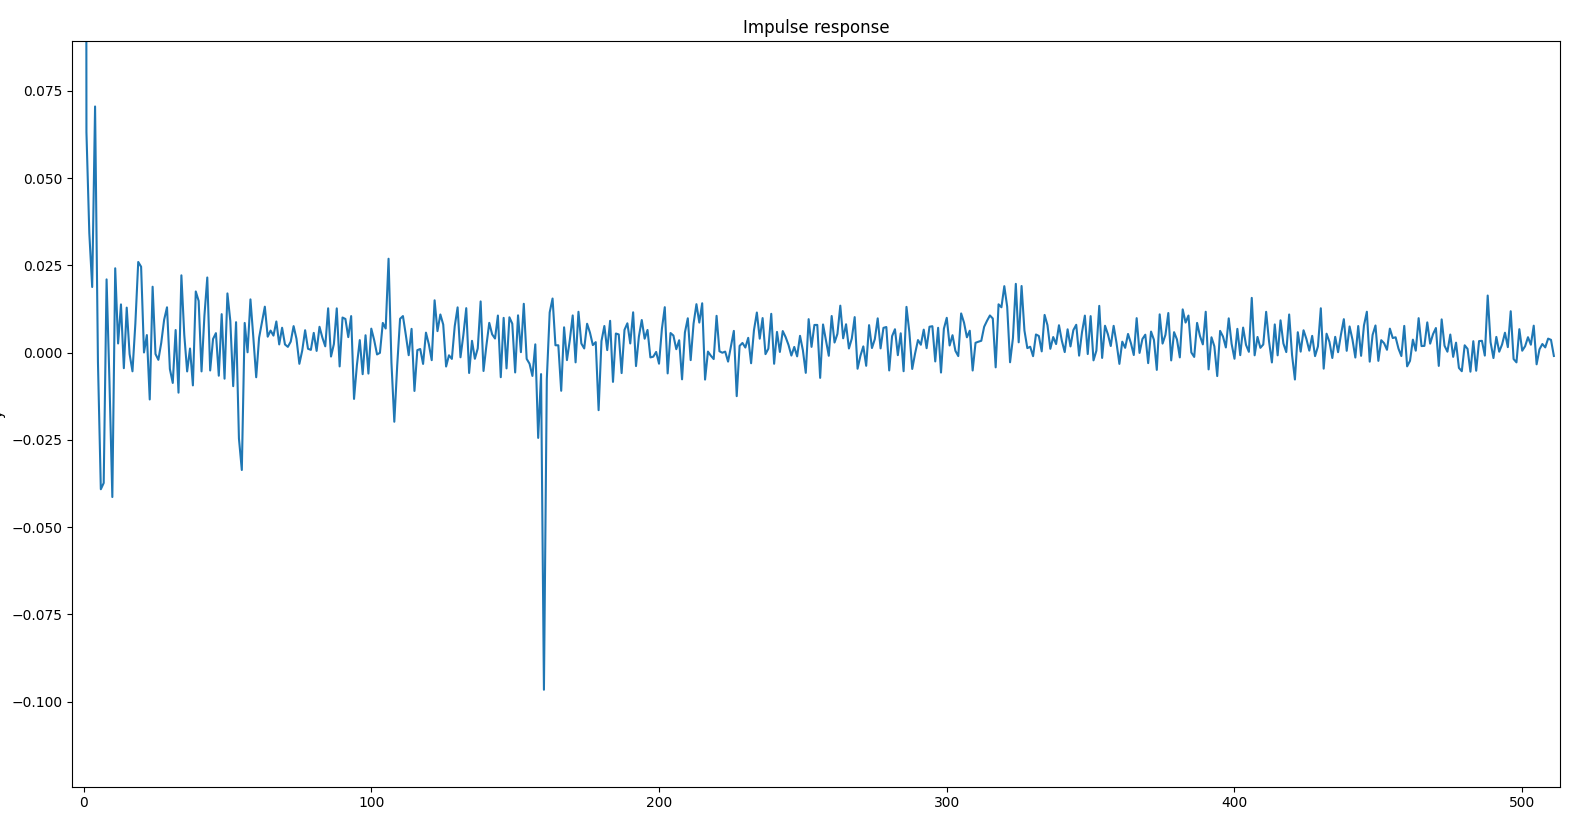
\includegraphics[scale=0.45]{images/Impulse_response.png}\hspace*{\fill}
\end{center}

\section{Simulace roušky}
\begin{center}
\hfill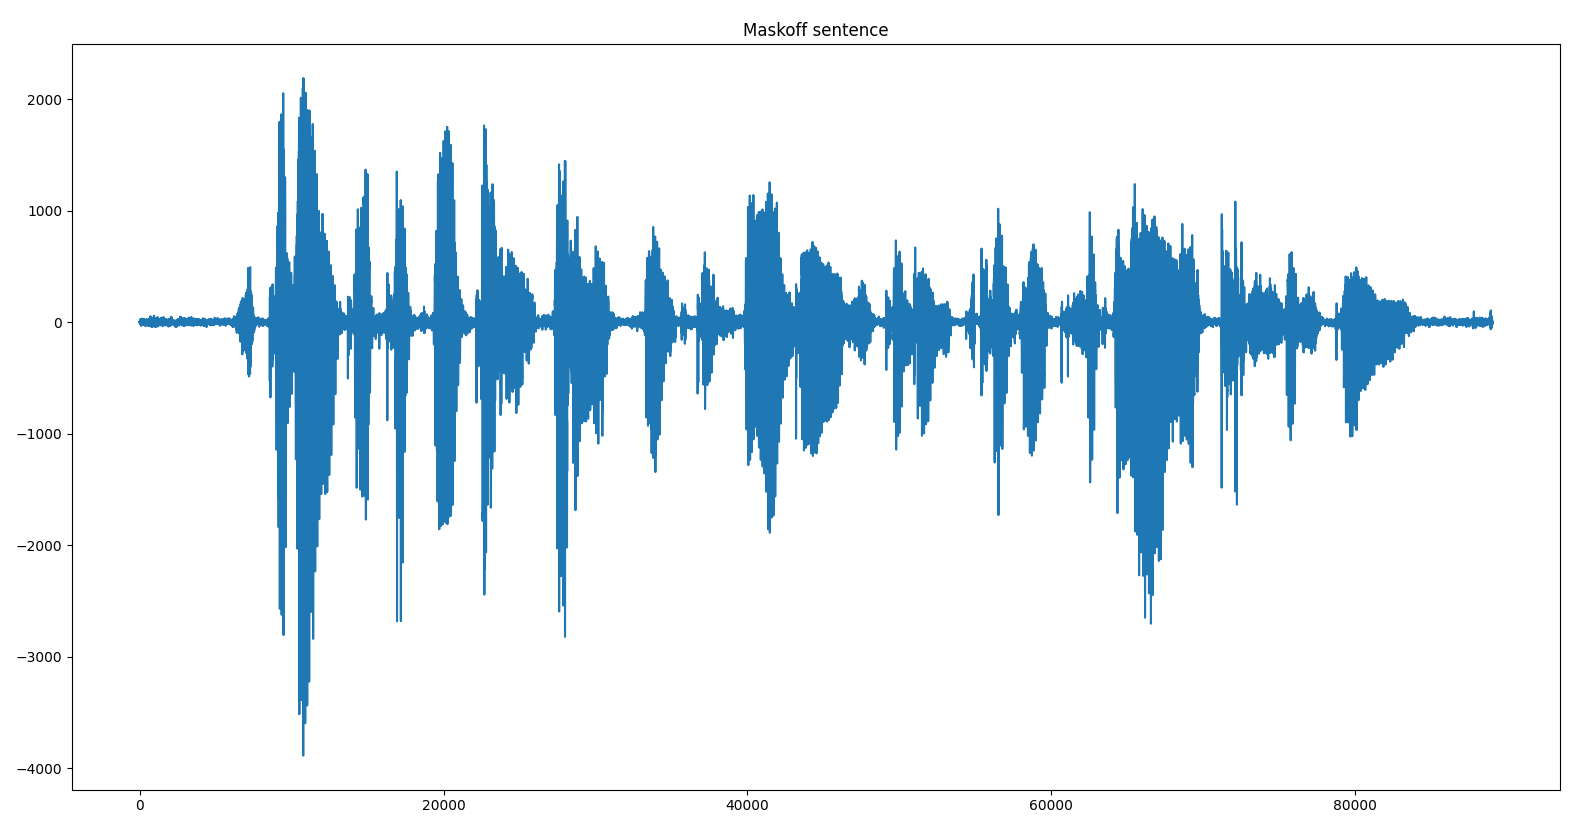
\includegraphics[scale=0.45]{images/Maskoff_sentence.png}\hspace*{\fill}
\end{center}
\begin{center}
\hfill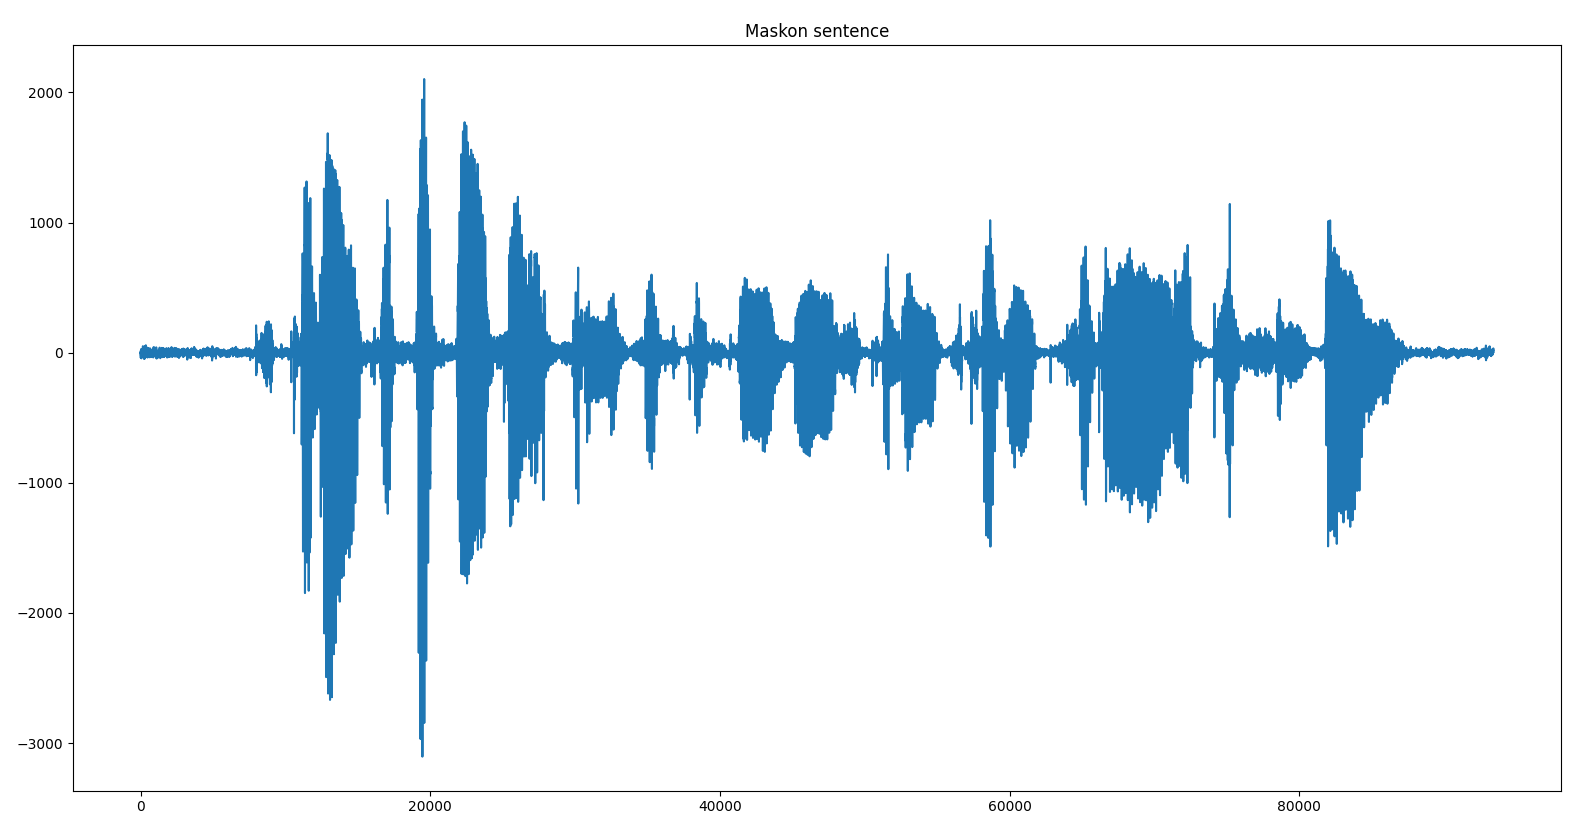
\includegraphics[scale=0.45]{images/Maskon_sentence.png}\hspace*{\fill}
\end{center}
\begin{center}
\hfill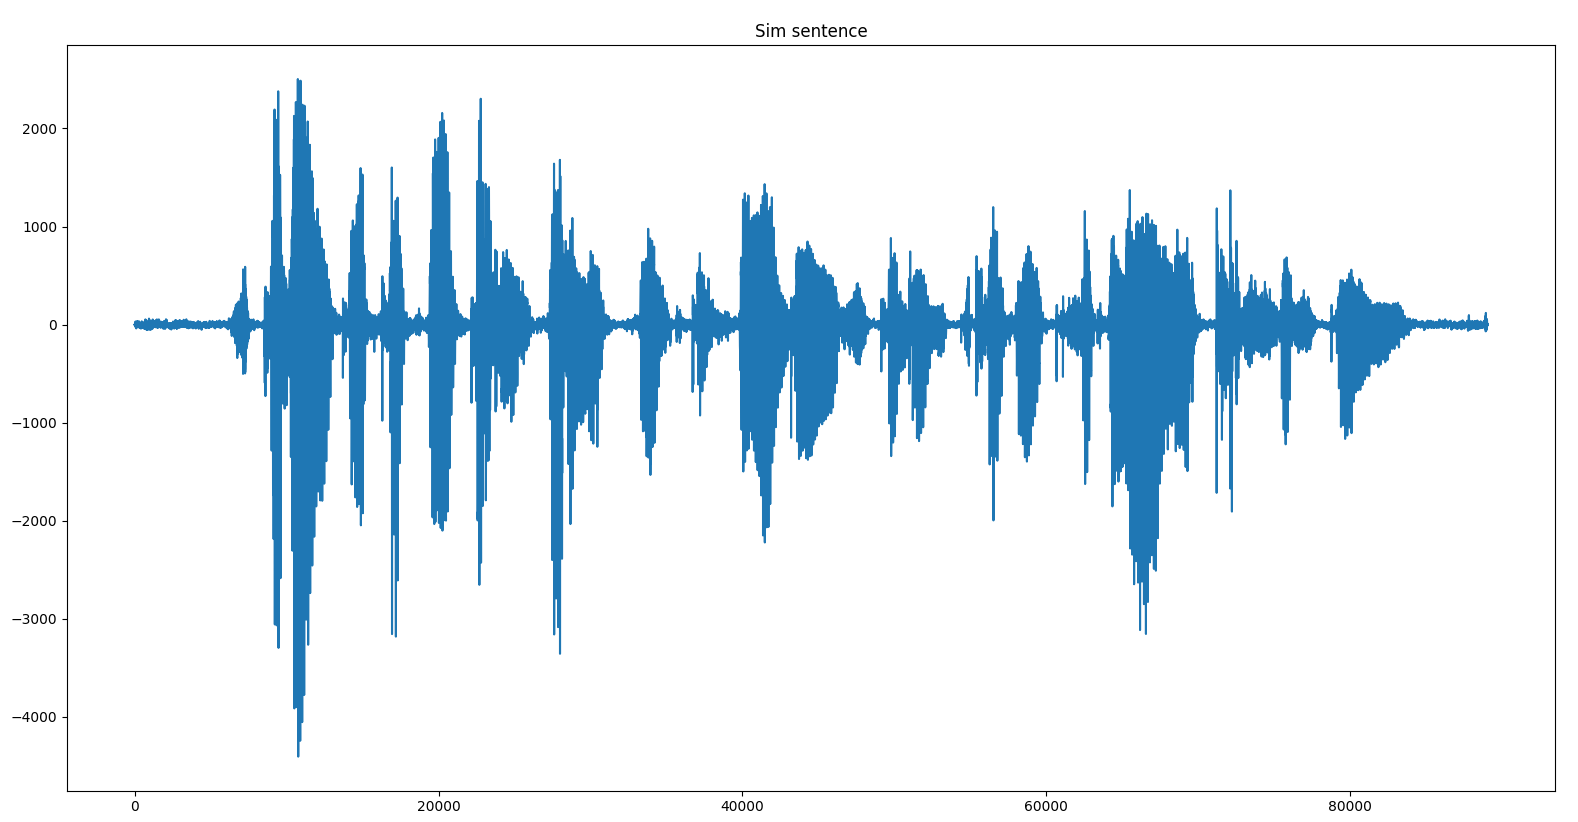
\includegraphics[scale=0.45]{images/Sim_sentence.png}\hspace*{\fill}
\end{center}

Simulovaná rouška se více podobá původnímu signálu bez roušky.

\section{Závěr}
Na začátku práce s projektem jsem odhadoval roušku na dolní propusť. Výsledná nahrávka simulované roušky je srozumitelná, nicméně není identická s originální rouškou, hlas je zašumělý. V průběhu výpočtu se počítalo s komplexními čísly a čísly s plovoucí řádovou čárkou, kde mohlo dojít ke zkreslení. Problém mohl vzniknout i při tvorbě nahrávek, které nebyly nahrány kvalitním mikrofonem a problémem držet jeden konkrétní tón. V průběhu zpracovávání protokolu musela být nahrávka několikrát vyměněna.
\end{document}

